\documentclass[sigplan,screen,10pt]{acmart}
\usepackage{circuitikz}
\usepackage{svg}
\usepackage{listings}

\lstset{
    basicstyle=\small\ttfamily,
	  keywordstyle=\ttfamily,
    columns=fullflexible,
    language=C,
    numbers=left,
    xleftmargin=18pt,
    stepnumber=1,
    breaklines=true,
    breakatwhitespace=true,
    showstringspaces=false,
    breaklines=true,
}

\settopmatter{printfolios=true,printccs=false,printacmref=false}
\renewcommand\footnotetextcopyrightpermission[1]{}

\pagestyle{plain} 

\begin{document}

\title{Flattening the Page Tables on Linux in x86\_64: Design, Implementation, and Evaluation in EMT Linux}

\author{Rubin Du}
\affiliation{
  \institution{University of Illinois at Urbana-Champaign}
}
\authornote{Both authors contributed equally.}
\email{rd25@illinois.edu}

\author{Shanbo Zhang}
\affiliation{
  \institution{University of Illinois at Urbana-Champaign}
}
\authornotemark[1]
\email{shanboz2@illinois.edu}

% \author{Siyuan Chai}
% \affiliation{
%   \institution{University of Illinois at Urbana-Champaign}
% }
% \email{siyuanc3@illinois.edu}

% \author{Tianyin Xu}
% \affiliation{
%   \institution{University of Illinois at Urbana-Champaign}
% }
% \email{tyxu@illinois.edu}

\begin{abstract}

    Virtual memory translation is a critical component of modern operating systems but often suffers from significant overhead due to deep multi-level page walks—particularly in the x86\_64 architecture. This overhead becomes a bottleneck for memory-intensive applications, especially under irregular access patterns found in data analytics, graph processing, and in-memory databases. In this work, we propose and implement a novel page table structure called the Flattened Page Table (FPT), which preserves the structure of hierarchical paging while enabling selective flattening of adjacent levels (e.g., L3-L2 or L4-L3+L2-L1). We integrate FPT into EMT-Linux \cite{emt} and modify both the kernel page table logic and QEMU to emulate hardware support for flattened walks. Our implementation supports multiple folding modes via kernel configuration and preserves backward compatibility with standard radix paging. Through a comprehensive evaluation using memory-intensive macro and application benchmarks, we show that FPT reduces kernel instruction overhead, improves instruction-per-cycle (IPC), and decreases page walk latency. These results demonstrate the feasibility and benefits of flattening page tables in commodity operating systems.

\end{abstract}


\maketitle

\section{Introduction}
\label{sec:introduction}

When the computing system was first invented, the memory was limited and expensive, and relevant logic was simple, because there were only one program running on the CPU. As time went on, the memory became larger and cheaper, and multiple users might run their programs on the same computers, but the CPU could only run one program at a time. The operating system should be able to take control of the CPU and manage the memory access of the user programs. Paging is a memory management scheme that eliminates the need for contiguous allocation of physical memory and creates the illusion to users of a very large (virtual) main memory. Paging scheme partitions the physical memory into fixed-size blocks called frames, and uses a table to map each virtual page to a physical frame. The page table contains information about each page.

Originally, the page table in x86 architecture is a two-level page table, where the address field in the first level points to the starting address of the second level page table, and the address field in the second level page table points to the starting address of the physical frame. Then, in x86\_64 architecture, the page table is extended to four levels. Later, it also supports 5-level page table extension. Typically, the page table is stored in memory due to its large size. For a memory access, in the worst case, the CPU needs to walk through all the levels of the page table to find the physical address. This is inefficient, and it could be the bottleneck of the system performance. Because of the popularity of machine learning, which consists of complex memory access patterns, the page table walking could be a performance bottleneck.

In this project, we implements a new page table structure called flattened page table (FPT). FPT maintains the logical behavior and interface of the traditional multi-level tree-structured page table, while enabling the selective flattening of adjacent levels to reduce the depth of the page table walk. Specifically, assuming the 5-level paging extension is not used, we support three folding modes: L4L3, L3L2, and L4L3-L2L1 folding. In each mode, the virtual address range covered by individual levels remains unchanged, but the number of levels traversed per walk is reduced by merging multiple levels into a single larger page table. The resulting structure remains logically hierarchical, but folded levels are stored as wider tables in memory, decreasing the number of required memory accesses for translation. Take L3L2 folding as an example. An L3 page table page is 4KB and maps a 1GB address space, and an L2 page table page is 4KB and maps a 2MB address space. In FPT L3L2 mode, however, the level 3 no longer exists, and L2 page table page is 2MB and maps a 1GB address space. Each entry in the L2 page table page points to an L1 page table page.

\section{Design}

\begin{figure}
    \centering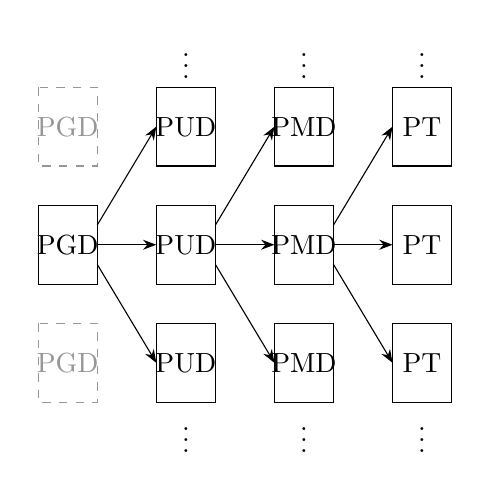
\begin{tikzpicture}[scale=0.5]
        \tikzstyle{every node}=[font=\normalsize]
        \draw  (0,0) rectangle  node {\normalsize PGD} (1.5,-2);
        \draw  (3,3) rectangle  node {\normalsize PUD} (4.5,1);
        \draw  (3,0) rectangle  node {\normalsize PUD} (4.5,-2);
        \draw  (3,-3) rectangle  node {\normalsize PUD} (4.5,-5);
        \draw [->, >=Stealth] (1.5,-0.5) -- (3,2);
        \draw [->, >=Stealth] (1.5,-1) -- (3,-1);
        \draw [->, >=Stealth] (1.5,-1.5) -- (3,-4);
        \draw  (6,3) rectangle  node {\normalsize PMD} (7.5,1);
        \draw  (6,0) rectangle  node {\normalsize PMD} (7.5,-2);
        \draw  (6,-3) rectangle  node {\normalsize PMD} (7.5,-5);
        \draw [->, >=Stealth] (4.5,-0.5) -- (6,2);
        \draw [->, >=Stealth] (4.5,-1) -- (6,-1);
        \draw [->, >=Stealth] (4.5,-1.5) -- (6,-4);
        \draw  (9,3) rectangle  node {\normalsize PT} (10.5,1);
        \draw  (9,0) rectangle  node {\normalsize PT} (10.5,-2);
        \draw  (9,-3) rectangle  node {\normalsize PT} (10.5,-5);
        \draw [->, >=Stealth] (7.5,-0.5) -- (9,2);
        \draw [->, >=Stealth] (7.5,-1) -- (9,-1);
        \draw [->, >=Stealth] (7.5,-1.5) -- (9,-4);
        \node [font=\normalsize] at (3.75,3.75) {$\vdots$};
        \node [font=\normalsize] at (3.75,-5.75) {$\vdots$};
        \node [font=\normalsize] at (6.75,3.75) {$\vdots$};
        \node [font=\normalsize] at (6.75,-5.75) {$\vdots$};
        \node [font=\normalsize] at (9.75,3.75) {$\vdots$};
        \node [font=\normalsize] at (9.75,-5.75) {$\vdots$};
        \draw [ color={rgb,255:red,150; green,150; blue,150} , dashed] (0,3) rectangle  node {\normalsize PGD}  (1.5,1);
        \draw [ color={rgb,255:red,150; green,150; blue,150} , dashed] (0,-3) rectangle  node {\normalsize PGD}  (1.5,-5);
    \end{tikzpicture}
    \caption{Traditional 4-level Radix Tree Strcuture in x86\_64}
    \Description{The radix tree structure in x86\_64. The radix tree is a tree data structure that stores the page table entries. Each node in the tree represents a level of the page table, and each edge represents a page table entry. The leaf nodes represent the physical frames.}
    \label{fig:radix_tree}
\end{figure}

\begin{figure}
    \centering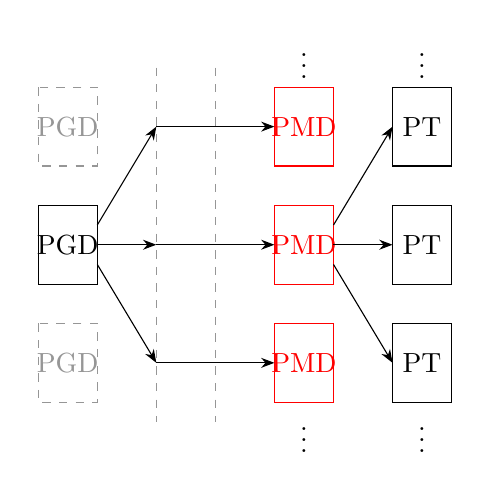
\begin{tikzpicture}[scale=0.5]
        \tikzstyle{every node}=[font=\normalsize]
        \draw  (0,0) rectangle  node {\normalsize PGD} (1.5,-2);
        \draw [->, >=Stealth] (1.5,-0.5) -- (3,2);
        \draw [->, >=Stealth] (1.5,-1) -- (3,-1);
        \draw [->, >=Stealth] (1.5,-1.5) -- (3,-4);
        \draw [ color={rgb,255:red,255; green,0; blue,0} ] (6,3) rectangle  node {\normalsize PMD} (7.5,1);
        \draw [ color={rgb,255:red,255; green,0; blue,0} ] (6,0) rectangle  node {\normalsize PMD} (7.5,-2);
        \draw [ color={rgb,255:red,255; green,0; blue,0} ] (6,-3) rectangle  node {\normalsize PMD} (7.5,-5);
        \draw  (9,3) rectangle  node {\normalsize PT} (10.5,1);
        \draw  (9,0) rectangle  node {\normalsize PT} (10.5,-2);
        \draw  (9,-3) rectangle  node {\normalsize PT} (10.5,-5);
        \draw [->, >=Stealth] (7.5,-0.5) -- (9,2);
        \draw [->, >=Stealth] (7.5,-1) -- (9,-1);
        \draw [->, >=Stealth] (7.5,-1.5) -- (9,-4);
        \node [font=\normalsize] at (6.75,3.75) {$\vdots$};
        \node [font=\normalsize] at (6.75,-5.75) {$\vdots$};
        \node [font=\normalsize] at (9.75,3.75) {$\vdots$};
        \node [font=\normalsize] at (9.75,-5.75) {$\vdots$};
        \draw [ color={rgb,255:red,150; green,150; blue,150} , dashed] (0,3) rectangle  node {\normalsize PGD}  (1.5,1);
        \draw [ color={rgb,255:red,150; green,150; blue,150} , dashed] (0,-3) rectangle  node {\normalsize PGD}  (1.5,-5);
        \draw [ color={rgb,255:red,150; green,150; blue,150}, dashed] (3,3.5) -- (3,-5.5);
        \draw [ color={rgb,255:red,150; green,150; blue,150}, dashed] (4.5,3.5) -- (4.5,-5.5);
        \draw [->, >=Stealth] (3,2) -- (6,2);
        \draw [->, >=Stealth] (3,-1) -- (6,-1);
        \draw [->, >=Stealth] (3,-4) -- (6,-4);
    \end{tikzpicture}
    \caption{Flattened Page Table (FPT) in L3L2 Mode}
    \Description{The flattened page table in L3L2 mode. The L3 level is folded into the L2 level, and the L2 level is enlarged to 2MB. The L2 level points to the L1 level.}
    \label{fig:folded_L3L2}
\end{figure}

Figure \ref{fig:radix_tree} shows the traditional 4-level radix tree structure in x86\_64. The radix tree is a tree data structure that stores the page table entries. Each node in the tree represents a level of the page table, and each edge represents a page table entry. The leaf nodes represent the physical frames. In the traditional 4-level radix tree structure, the uppermost level (L4) is the Page Global Directory (PGD), which points to the Page Upper Directory (PUD, L3). The PUD points to the Page Middle Directory (PMD, L2), and the PMD points to the Page Table (PT, L1). The PT points to the physical frames. In our design, we enables some level(s) of tables to be flattened. The lower level now spans the virtual address space spanned by the folded levels, but the size of the folded level(s) table is increased (from 4KB to 2MB). Take L3L2 folding as an example. An L3 page table page is 4KB and maps a 1GB address space; an L2 page table page is 4KB and maps a 2MB address space. In FPT L3L2 mode, however, the level 3 no longer exists, and L2 page table page is 2MB and maps a 1GB address space. Each entry in the L2 page table page points to an L1 page table page. Figure \ref{fig:folded_L3L2} shows the flattened page table in L3L2 mode. The PUD level no longer exists (even in hardware), and the PMD level (marked as red) is enlarged to 2MB.
\section{Implementation}

% \subsection{Basics and Overview}

In this section, we will discuss the implementation of the FPT in Linux. Since x86\_64 is a complex architecture, and it is not open-source, we can only emulate the behavior of the FPT mechanism in Linux by emulators. We modified QEMU with version 6.1.50 to support the FPT mechanism in ``hardware''. We also used Linux kernel version 5.15.0 to support the FPT mechanism. We changed the kernel to support the FPT mechanism by modifying the logic for page allocation logic, page table walk logic, and some TLB logic.

Before we start to discuss the implementation, we need to activate the FPT mechanism in the kernel. The FPT mechanism is not enabled by default in the kernel, but allowed by some new Kconfig options - one for enabling the FPT mechanism and one for selecting the folding level, as we mentioned before. The configuration becomes effective in the kernel image after the kernel is compiled with the new Kconfig options. We retain the backward compatibility with the radix structure, and the kernel could jump to suitable routines based on the enabled configuration.

\subsection{EMT TEntry and Iterator Logic}

The EMT Linux uses tentry struct to optimize the logic of reading, inserting, and updating a page table entry at a given address. It also comes with an iterator to reduce the overhead of traversing the page table. To accomodate for FPT, the tentry struct will ignore folded level and skip to next level, and the iterator it need to check whether the currently iterating page table is flattened or not, and align the address iterator to the same granularity as the page table when initializing the iterator from address, or finding next address to check.

\subsection{Page Allocation Logic}

The page allocation logic is responsible for allocating physical pages to the virtual address space of a process. The Linux kernel uses a buddy allocator to allocate physical pages. We do not need to modify the buddy allocator, but we need to modify the page allocation logic to support the FPT mechanism. Traditionally, the page table pages in each level have size 4KB. The kernel uses \lstinline|struct page| to represent a 4KB page frame, and contiguous \lstinline|struct page| maps to physically contiguous address space. In FPT, however, the page table pages of the flattened level could have size 2MB. Hence, we need to modify the page allocation logic to check the level we are allocating the page table. If the level is the flattened level, we need to allocate a contiguous address space of 2MB, which corresponds to 512 ($2^9$) \lstinline|struct page| objects. To achieve that, the generic EMT interface of \lstinline|create_context| and \lstinline|insert_tentry| is overridden with fpt specific version, which upon allocating a page, checks if the respective level is folded into its next level, if not, it will attempt to allocate a 2MB page using \lstinline|get_free_pages| with order of 9, if that was not possible due to that flattening this level was disabled by kernel config flags, or allocation of a order 9 page failed, it will allocate a 4KB page.After that, it will set the folded bit of the entry of that page to reflect whether it is a flattened page or not, to be used in translation and deallocation.

\subsection{Page Table Walk Logic}

The page table lookup logic is responsible for translating a virtual address to a physical address. The Linux kernel uses a multi-level page table structure to perform this translation. In FPT, the page table structure is flattened, which means that some levels of the page table are folded into the next level. This requires modifying the page table lookup logic to handle the flattened levels correctly. The translation happening on the hardware path mainly utilizes the flattened bit to determine whether to use 9 bits or 18 bits to index the next level. On the software path, the generic EMT interface of \lstinline|p*d_offset_map_with_mm| is overriden with \lstinline|fpt_p*d_offset_map_with_mm|, which checks kernel config and the respective flatten bit of the PT entry, to correctly compute the pointer to the next level of the page table. For example, if the system calls \lstinline|pmd_offset_map_with_mm| via EMT, it will check the kernel config flags and the pud entry to see if pmd is folded into pte, if so it will simply return original pud entry, which can be used as a pmd entry to get pte via its next level translation interface. If not, it will then check if pud is folded into pmd, if so it will use 18 bits in the address to traverse the pmd table to find the correct entry, else it will do a normal pmd lookup.

\subsection{Page Table Free Logic}

The page table deallocation logic is responsible for freeing the physical pages that are no longer needed. In FPT, the page table deallocation logic needs to be modified to handle the flattened levels, as well as the use of mixed flattened and normal page tables correctly. The deallocation logic is similar to the reverse of the allocation logic, first it uses \lstinline|unmap_vmas| to unmap and deallocate leaf pages, which uses the EMT tentry iterators to iterate over page tables to free all leaf pages. After that it will call \lstinline|free_pgtables| to deallocate all page tables, which recursively scans from the top to lowest pagetable levels and deallocate all page tables fully covered from the vma's start to end address. In FPT this is modified to check if its the scanning level is folded, normal, or flattened. If folded it will simply pass all parameters to its next level, if normal it will follow radix deallocation logic, and if flattened it will scan over 2MB range and call next level deallocation logic for each entry, and if all is freed and within the vma's range, it will delete its entry from its parent's parent level. When a page table is throughly freed, also it need to invalidate itself from TLB using \lstinline|p*d_free_tlb| and release the page back to the buddy allocator, if the page is flattened this will invalidate the range its parent cover from TLB, and free a order 9 page.

\subsection{TLB Logic}

TLB, or Translation Lookaside Buffer, is a hardware cache that stores the most recently used page table entries. The TLB is used to speed up the translation of virtual addresses to physical addresses. Flushing the TLB is a process of invalidating the TLB entries to ensure that the TLB does not contain stale entries. In Linux kernel, the TLB flush is associated with \lstinline|struct page|, too. Since flushing the TLB is an expensive operation, the Linux kernel batches page frames to be flushed, until the batched list reaches some certain threshold. Nevertheless, in FPT, everytime we release a flattened page table page, there will be 512 ($2^9$) pages to be flushed, which is higher than all possible existing thresholds. Hence, we need to modify the TLB flush logic to support the FPT mechanism. Currently, our design is to enforce a TLB flush if some flattened page table pages are being released, which also helps release the pages existing in the batched list. This might not be a best design. Some improvements could be made in the future. For example, we could reprogram the existing TLB interfances to accommondate the changing page sizes (because we found some routines accept the \lstinline|struct page| only, but not the size or the order). We could also change the policy to trigger a TLB flush, design a specialized TLB interface for the FPT mechanism, or even further polish the hardware structure of TLB.

\subsection{Page Fault Handling Logic}

The page fault handling logic is essentially same to radix, the only changes are the modifications to EMT iterators to align to the flattened page size when iterating over vmfs.
\section{Evaluation}

In this section, we evaluate the performance of our implementation of the flattened page table in Linux. We first present the experimental setup, including the hardware and software configurations. Then, we compare the performance of our implementation with the original 4-level radix paging mechanism, and the ECPT paging mechanism in Linux using various benchmarks. Finally, we analyze the results and discuss the implications of our findings.

% TODO: add reference for ECPT, csynb

\subsection{Methodology and Metrics}

To evaluate the performance of our Flattened Page Table (FPT) implementation, we designed a comprehensive evaluation pipeline that executes benchmarks inside QEMU virtual machines, collects low-level memory traces, and performs offline analysis using instrumentation and custom tooling. Our methodology ensures consistency and fairness when comparing FPT against the baseline 4-level Radix Tree paging and the ECPT mechanism.

We run various benchmarks inside QEMU virtual machines with different configurations, including the original 4-level radix paging, the ECPT mechanism, and two configurations, L3L2 mode and L4L3+L2L1 mode, of our FPT implementation. The benchmarks include a mix of workloads that stress different aspects of the memory management system, such as memory allocation, page table lookups, and memory-intensive applications. For each benchmark, we split the execution into loading and running phases. The loading phase is used to load the benchmark into memory, while the running phase is used to execute the benchmark. We measure the execution time of each phase separately to understand the impact of our FPT implementation on both loading and running times.

During executing the benchmarks, we collect low-level memory traces using DynamoRIO, a dynamic binary instrumentation framework. We collect information about memory accesses, page walk latencies, TLB misses, instruction counts, and some other performance metrics. We then generate some visualization graphs to help partition the memory access of each execution of benchmarks and compare the performance of the different configurations.

\subsection{Benchmarks}

We selected a diverse set of benchmarks to evaluate the performance of our FPT implementation.

We use seven memory-intensive macro benchmarks. Some benchmarks are selected from the GraphBIG benchmark suite, which is a collection of graph processing workloads. The benchmarks include: 
    Breadth-First Search (BFS),
    Depth-First Search (DFS),
    Degree Centruality (DC),
    Single-Source Shortest Path (SSSP),
    Connected Components (CC),
    Triangle Counting (TC),
    PageRank (PR).

We also run the GUPS benchmark for random memory access, and a memory test from SysBench. Both benchmarks have 64GB working sets.

\begin{table}
    \centering
    \footnotesize
    \setlength{\tabcolsep}{2pt}
    \begin{tabular}{lcccc}
        \toprule
        \textbf{Application} & \textbf{Working Set} & {\bf \# Records} & \textbf{Read:Write} & {\bf \# Requests} \\
        \midrule
        Redis      & 128 GB & 536 M & 50:50 & 60 M \\
        Memcached  & 69 GB  & 56 M  & 80:20 &  10 M \\
        PostgreSQL & 64 GB  & 21 M & 100:0 & 25 M \\
        \bottomrule
    \end{tabular}
    \caption{\bf Application workloads used in the evaluation.}
    \label{table:workloads}
\end{table}

\begin{figure}
    \centering
    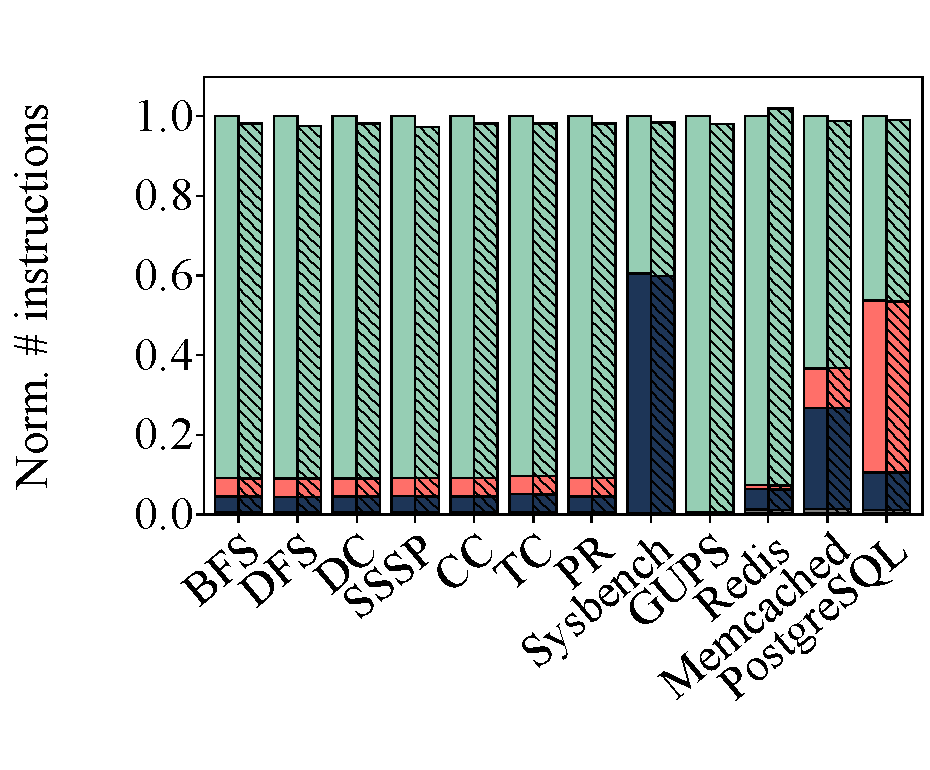
\includegraphics[width=0.495\linewidth]{graph/kern_inst_unified_never_L3L2.pdf} 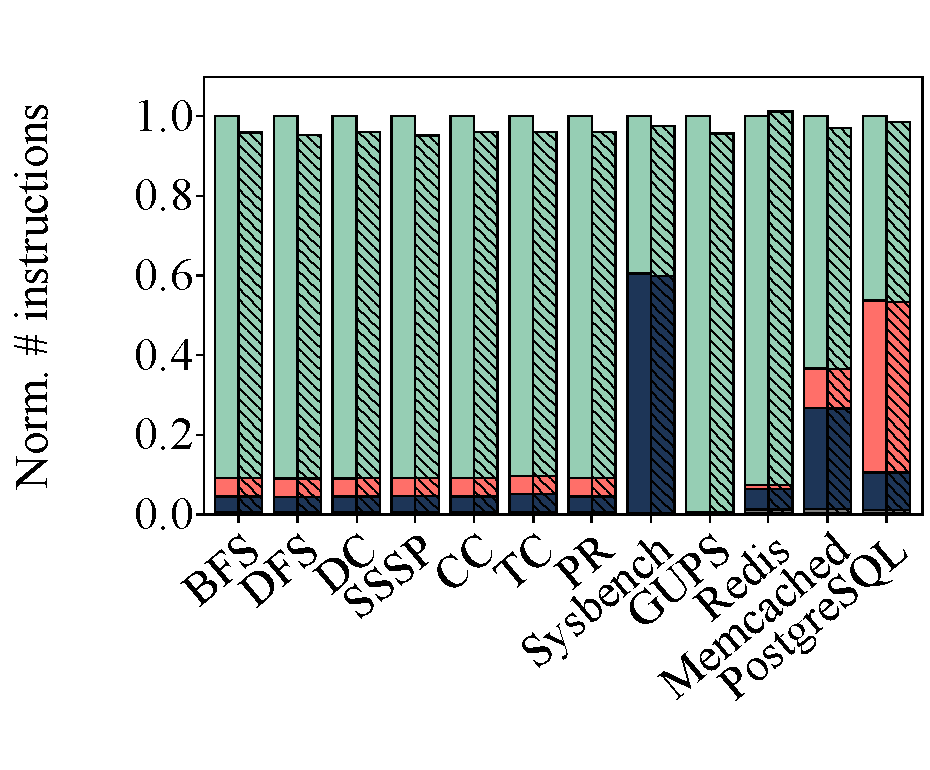
\includegraphics[width=0.495\linewidth]{graph/kern_inst_unified_never_L4L3L2L1.pdf}
    \caption{Distribution of kernel instructions of EMT-Linux with the Radix and FPT L3L2 mode (left) and L4L3+L2L1 mode (right).}
    \label{fig:kernel_inst}
\end{figure}

We also keep track of three memory-intensive real-world applications:
    Redis,
    Memcached,
    PostgreSQL.
Table \ref{table:workloads} summarizes the workloads of these applications.

% TODO: citation for GraphBIG

\subsection{Results}

\subsubsection{OS Overhead of FPT}

Figure~\ref{fig:kernel_inst} shows the distribution of kernel instructions under the Radix paging and two Flattened Page Table (FPT) configurations: L3L2 mode (left) and L4L3+L2L1 mode (right). The shaded areas represent instructions executed under FPT modes, while the blue, red, green, and gray segments correspond to instructions related to timers, system calls, page faults, and other kernel activities, respectively. Compared to the Radix baseline, both FPT modes show a slight reduction in the total number of kernel instructions, with a more noticeable decrease in the L4L3+L2L1 configuration.

We believe that the reduction in kernel instructions is primarily due to the decreased number of page table walks and TLB misses. The kernel instruction reduction in L4L3+L2L1 mode could be because the L4L3+L2L1 mode reduces one more page table level that need to be traversed during address translation, leading to fewer kernel instructions related to page table lookups. Overall, these results demonstrate that FPT, especially the more aggressive L4L3+L2L1 mode, can alleviate kernel instruction overhead and improve execution efficiency for memory-intensive applications.

\subsubsection{Performance Comparison}

\begin{figure}
    \centering
    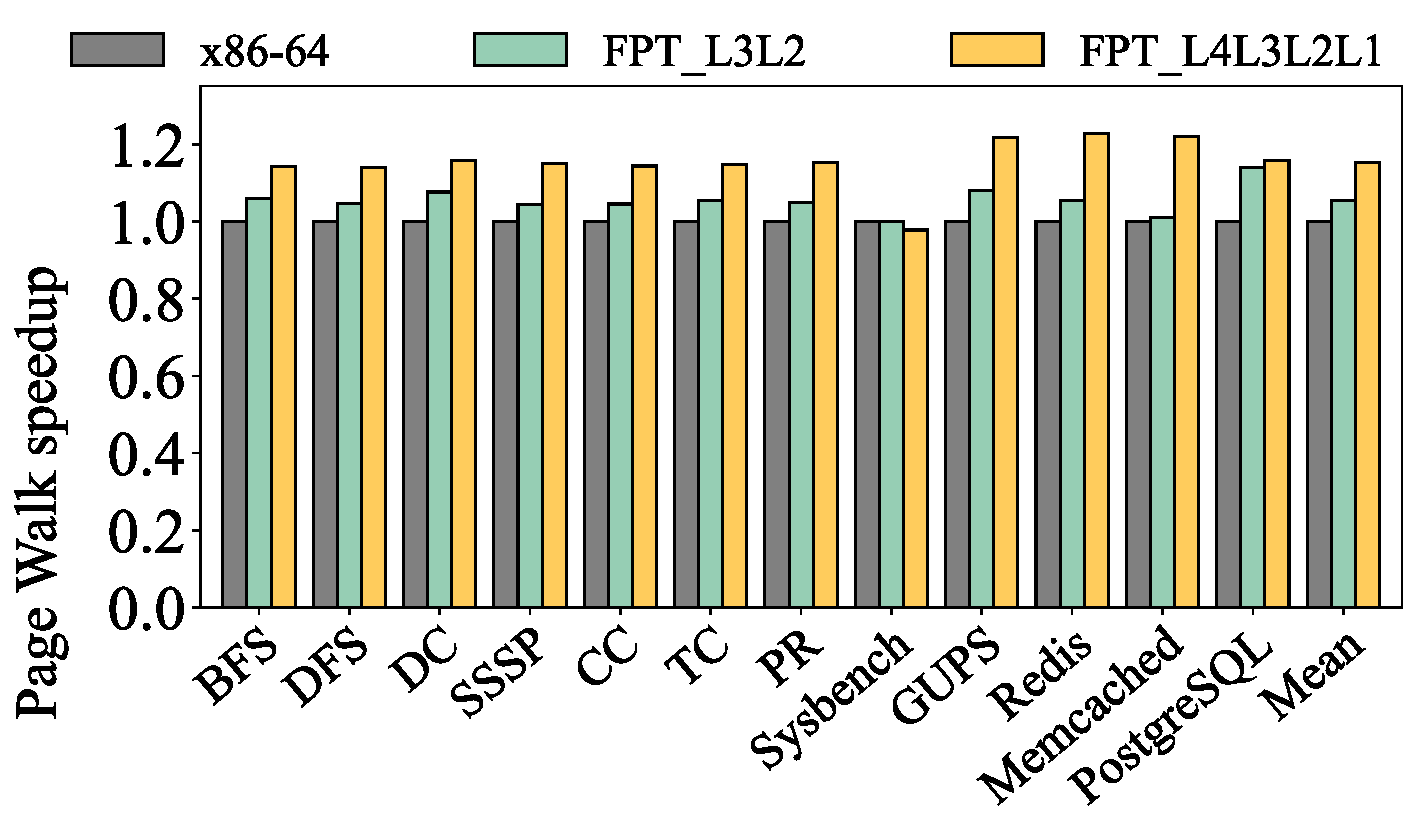
\includegraphics[width=0.85\linewidth]{graph/fpt_pgwalk_unified_never.pdf}
    \caption{Page Walk Latencies of Radix and FPT modes}
    \label{fig:fptpgwalk}
\end{figure}

\begin{figure}
    \centering
    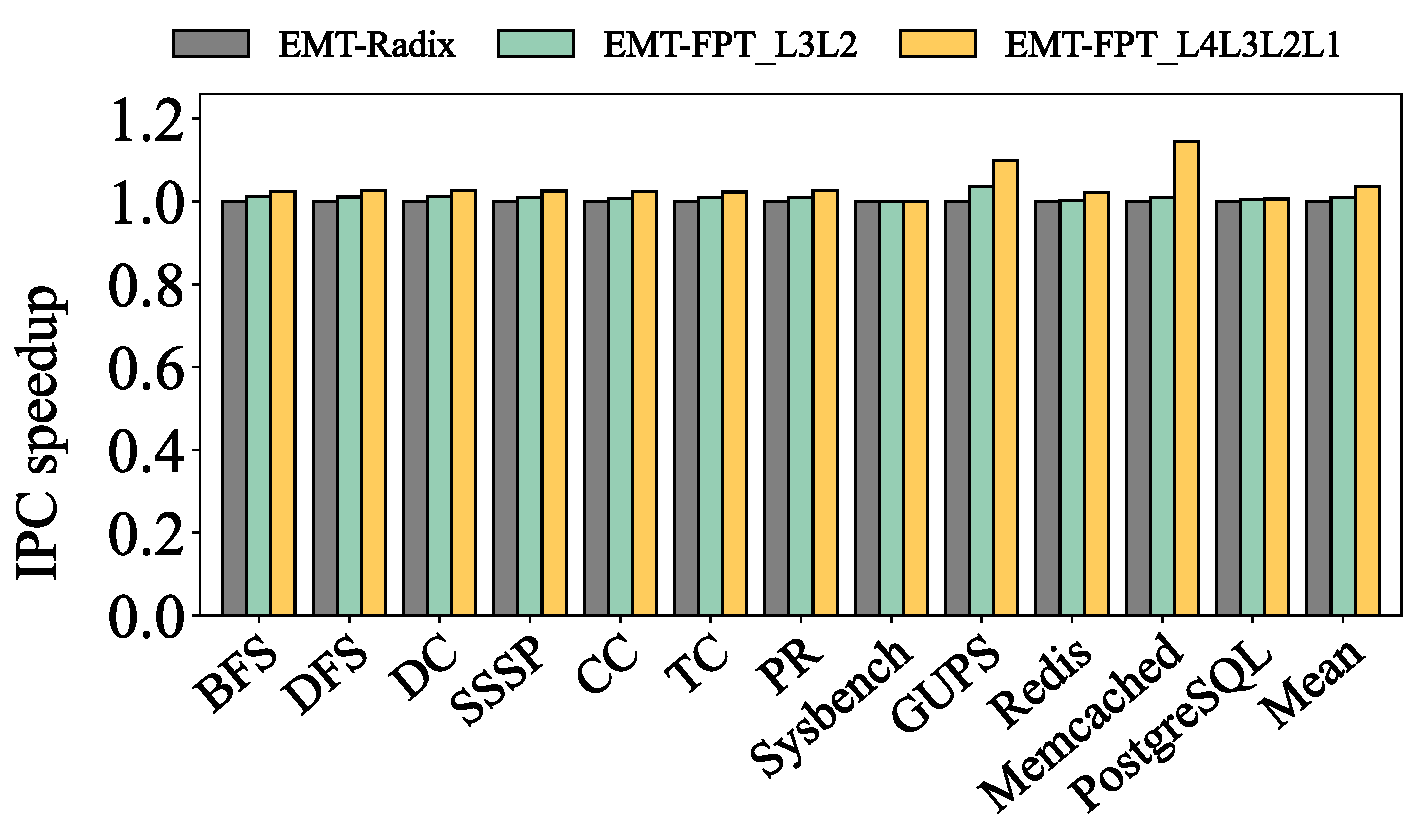
\includegraphics[width=0.85\linewidth]{graph/fpt_ipc_unified_never.pdf}
    \caption{IPC Speedup of Radix and FPT modes}
    \label{fig:fptipc}
\end{figure}

\begin{figure}
    \centering
    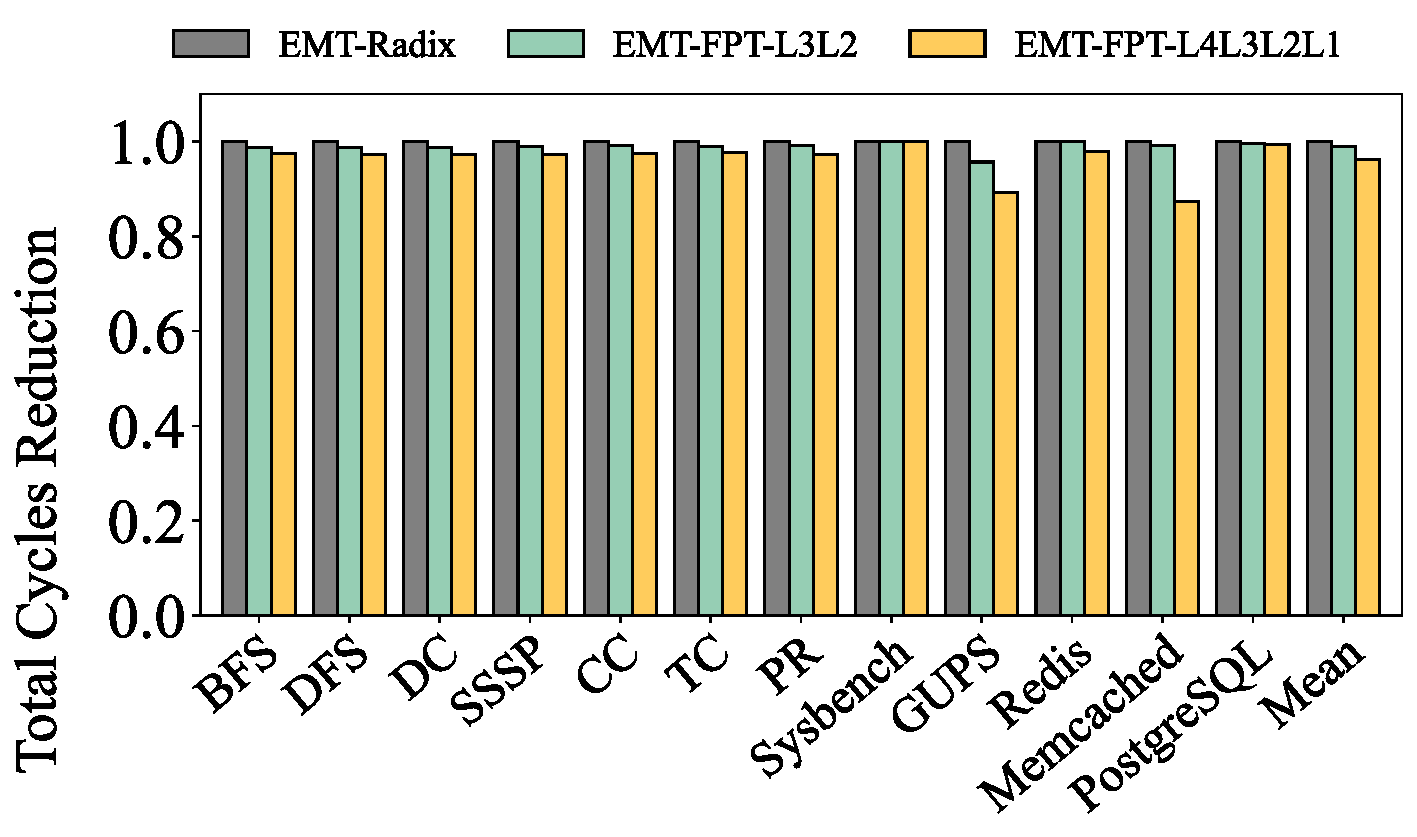
\includegraphics[width=0.85\linewidth]{graph/fpt_e2e_unified_never.pdf}
    \caption{End-to-End Latency of Radix and FPT modes}
    \label{fig:fpte2e}
\end{figure}


\section{Related Work}



\section{Conclusion}

This work presented the Flattened Page Table (FPT), a practical modification to the x86\_64 Linux memory management subsystem that reduces virtual-to-physical address translation overhead by selectively collapsing levels of the page table hierarchy. By merging adjacent levels—such as L3L2 or L4L3+L2L1—into wider tables, FPT shortens the translation path while maintaining compatibility with existing software and hardware expectations. We implemented FPT in EMT-Linux and extended QEMU to emulate the required hardware behavior, enabling end-to-end support for flattened page walks.

Our evaluation demonstrates that FPT leads to measurable reductions in kernel instruction counts, page walk latency, and overall execution time on memory-intensive workloads, outperforming both standard radix paging and Elastic Cuckoo Page Tables (ECPT) in several cases. These results suggest that even modest changes to the page table layout can bring substantial benefits. FPT serves as a promising direction for future systems that seek to optimize address translation with minimal disruption to existing software ecosystems.

\section{Metadata}

The presentation of the project can be found at:
\begin{center}
\fbox{\url{https://zoom/cloud/link/}}
\end{center}

\noindent
The code/data of the project can be found at:

\begin{center}
\fbox{\url{https://github.com/xlab-uiuc/linux_gen}} \\
\fbox{\url{https://github.com/xlab-uiuc/dynamorio}} \\
\fbox{\url{https://github.com/xlab-uiuc/VM-Bench}} \\
\end{center}


\bibliographystyle{acm}
\bibliography{ref}

\end{document}
\endinput
